    For this problem,
    \begin{align}
        \vec{x} = \vec{x_2} - \vec{x_1} = \myvec{3\\3\\3} \\
        \vec{M} = \myvec{\vec{m_1} & \vec{m_2}} = \myvec{1&2\\-3&3\\2&1} 
    \end{align}
    Thus,
    \begin{align}
        \vec{M}^\top\vec{M} = \myvec{1&-3&2\\2&3&1}\myvec{1&2\\-3&3\\2&1} = \myvec{14&-5\\-5&14} \\
        \vec{MM}^\top = \myvec{1&2\\-3&3\\2&1}\myvec{1&-3&2\\2&3&1} = \myvec{5&3&4\\3&18&-3\\4&-3&5}
    \end{align}
    We perform the eigendecompositions for each matrix and bring them into the form
    \begin{align}
        \vec{MM}^\top &= \vec{P_1D_1P_1}^\top \label{eq:chapters/12/11/2/16/svd/decomp-1} \\
        \vec{M}^\top\vec{M} &= \vec{P_2D_2P_2}^\top \label{eq:chapters/12/11/2/16/svd/decomp-2}
    \end{align}
    \begin{enumerate}
        \item For $\vec{MM}^\top$, the characteristic polynomial is
        \begin{align}
		\text{char}{\vec{MM}^\top} &= \mydet{x-5&-3&-4\\-3&x-18&3\\-4&3&x-5} \\
                                      &= x\brak{x-9}\brak{x-19}
                                      \label{eq:chapters/12/11/2/16/svd/char-2}
        \end{align}
        Thus, the eigenvalues are given by
        \begin{align}
            \lambda_1 = 19,\ \lambda_2 = 9,\ \lambda_3 = 0
        \end{align}
        For $\lambda_1$, the augmented matrix formed from the 
        eigenvalue-eigenvector equation is
        \begin{align}
            &\myvec{-14&3&4&0\\3&-1&-3&0\\4&-3&-14&0} \nonumber \\
            &\xleftrightarrow[]{R_1 \leftarrow \frac{R_1+R_3}{-10}} \myvec{1&0&1&0\\3&-1&-3&0\\4&-3&-14&0} \\
            &\xleftrightarrow[]{R_2 \leftarrow -R_2+3R_1} \myvec{1&0&1&0\\0&1&6&0\\4&-3&-14&0} \\
            &\xleftrightarrow[]{R_3 \leftarrow R_3-4R_1} \myvec{1&0&1&0\\0&-1&-6&0\\0&-3&-18&0} \\
            &\xleftrightarrow[]{R_3 \leftarrow R_3-3R_2} \myvec{1&0&1&0\\0&-1&-6&0\\0&0&0&0}
        \end{align}
        Hence, the normalized eigenvector is
        \begin{align}
            \vec{p_1} = \frac{1}{\sqrt{38}}\myvec{-1\\-6\\1}
        \end{align}
        For $\lambda_2$, the augmented matrix formed from the 
        eigenvalue-eigenvector equation is
        \begin{align}
            &\myvec{-4&3&4&0\\3&9&-3&0\\4&3&-4&0} \nonumber \\
            &\xleftrightarrow[]{R_3 \leftarrow R_1+R_3} \myvec{-4&3&4&0\\3&9&-3&0\\0&0&0&0} \\
            &\xleftrightarrow[]{R_2 \leftarrow \frac{4R_2+3R_1}{45}} \myvec{-4&3&4&0\\0&1&0&0\\0&0&0&0} \\
            &\xleftrightarrow[]{R_1 \leftarrow \frac{R_1-3R_2}{-4}} \myvec{1&0&-1&0\\0&1&0&0\\0&0&0&0}
        \end{align}
        Hence, the normalized eigenvector is
        \begin{align}
            \vec{p_2} = \frac{1}{\sqrt{2}}\myvec{1\\0\\1}
        \end{align}
        For $\lambda_3$, the augmented matrix formed from the 
        eigenvalue-eigenvector equation is
        \begin{align}
            &\myvec{5&3&4&0\\3&18&-3&0\\4&-3&5&0} \nonumber \\ 
            &\xleftrightarrow[]{R_1 \leftarrow \frac{R_1+R_3}{9}} \myvec{1&0&1&0\\3&18&-3&0\\4&-3&5&0} \\
            &\xleftrightarrow[]{R_2 \leftarrow R_2-3R_1} \myvec{1&0&1&0\\0&18&-6&0\\4&-3&5&0} \\
            &\xleftrightarrow[]{R_3 \leftarrow R_3-4R_1} \myvec{1&0&1&0\\0&18&-6&0\\0&-3&1&0} \\
            &\xleftrightarrow[]{R_2 \leftarrow \frac{R_2}{6}} \myvec{1&0&1&0\\0&3&-1&0\\0&-3&1&0} \\
            &\xleftrightarrow[]{R_3 \leftarrow R_3+R_2} \myvec{1&0&1&0\\0&3&-1&0\\0&0&0&0}
        \end{align}
        Hence, the normalized eigenvector is
        \begin{align}
            \vec{p_3} = \frac{1}{\sqrt{19}}\myvec{-3\\1\\3}
        \end{align}
        Using \eqref{eq:chapters/12/11/2/16/svd/decomp-1}, we see that
        \begin{align}
            \vec{P_1} = \myvec{-\frac{1}{\sqrt{38}}&\frac{1}{\sqrt{2}}&-\frac{3}{\sqrt{19}}\\-\frac{6}{\sqrt{38}}&0&\frac{1}{\sqrt{19}}\\\frac{1}{\sqrt{38}}&-\frac{1}{\sqrt{2}}&\frac{3}{\sqrt{19}}} \\
            \vec{D_1} = \myvec{19&0&0\\0&9&0\\0&0&0}
            \label{eq:chapters/12/11/2/16/svd/eig-params-1}
        \end{align}
        \item For $\vec{M}^\top\vec{M}$, the characteristic polynomial is
        \begin{align}
		\text{char}{\vec{M}^\top\vec{M}} &= \mydet{x-14&5\\5&x-14} \\
                                      &= \brak{x-9}\brak{x-19}
%                                      \label{eq:chapters/12/11/2/16/svd/char-1}
        \end{align}
        Thus, the eigenvalues are given by
        \begin{align}
            \lambda_1 = 19,\ \lambda_2 = 9
        \end{align}
        For $\lambda_1$, the augmented matrix formed from the 
        eigenvalue-eigenvector equation is
        \begin{align}
            \myvec{-5&-5&0\\-5&-5&0} &\xleftrightarrow[]{R_1 \leftarrow R_1-R_2} \myvec{0&0&0\\-5&-5&0}
        \end{align}
        Hence, the normalized eigenvector is
        \begin{align}
            \vec{p_1} = \frac{1}{\sqrt{2}}\myvec{1\\-1}
        \end{align}
        For $\lambda_2$, the augmented matrix formed from the 
        eigenvalue-eigenvector equation is
        \begin{align}
            \myvec{5&-5&0\\-5&5&0} &\xleftrightarrow[]{R_1 \leftarrow R_1+R_2} \myvec{0&0&0\\5&-5&0}
        \end{align}
        Hence, the normalized eigenvector is
        \begin{align}
            \vec{p_2} = \frac{1}{\sqrt{2}}\myvec{1\\1}
        \end{align}
        Thus, from \eqref{eq:chapters/12/11/2/16/svd/decomp-2},
        \begin{align}
            \vec{P_2} = \myvec{\frac{1}{\sqrt{2}}&-\frac{1}{\sqrt{2}}\\\frac{1}{\sqrt{2}}&\frac{1}{\sqrt{2}}},\ \vec{D_2} = \myvec{9&0\\0&19}
            \label{eq:chapters/12/11/2/16/svd/eig-params-2}
        \end{align}
    \end{enumerate}
    Therefore, from \eqref{eq:chapters/12/11/2/16/svd/M-svd},
    \begin{align}
        \vec{U} &= \vec{P_1} \\ 
        \vec{V} &= \vec{P_2} \\
        \vec{\Sigma} &= \myvec{\sqrt{19}&0\\0&3\\0&0}
        \label{eq:chapters/12/11/2/16/svd/svd-params}
    \end{align}
    and substituting into \eqref{eq:chapters/12/11/2/16/svd/lambda-sol}, we get
    \begin{align}
        \vec{\lambda} = \frac{1}{19}\myvec{10\\28}
    \end{align}
    which agrees with earlier solutions as well.
    \iffalse
    The Python code
    \texttt{codes/svd.py} plots 
    \fi
    See Fig. \ref{fig:chapters/12/11/2/16/svd/svd} depicting the situation.
    \begin{figure}[!ht]
        \centering
        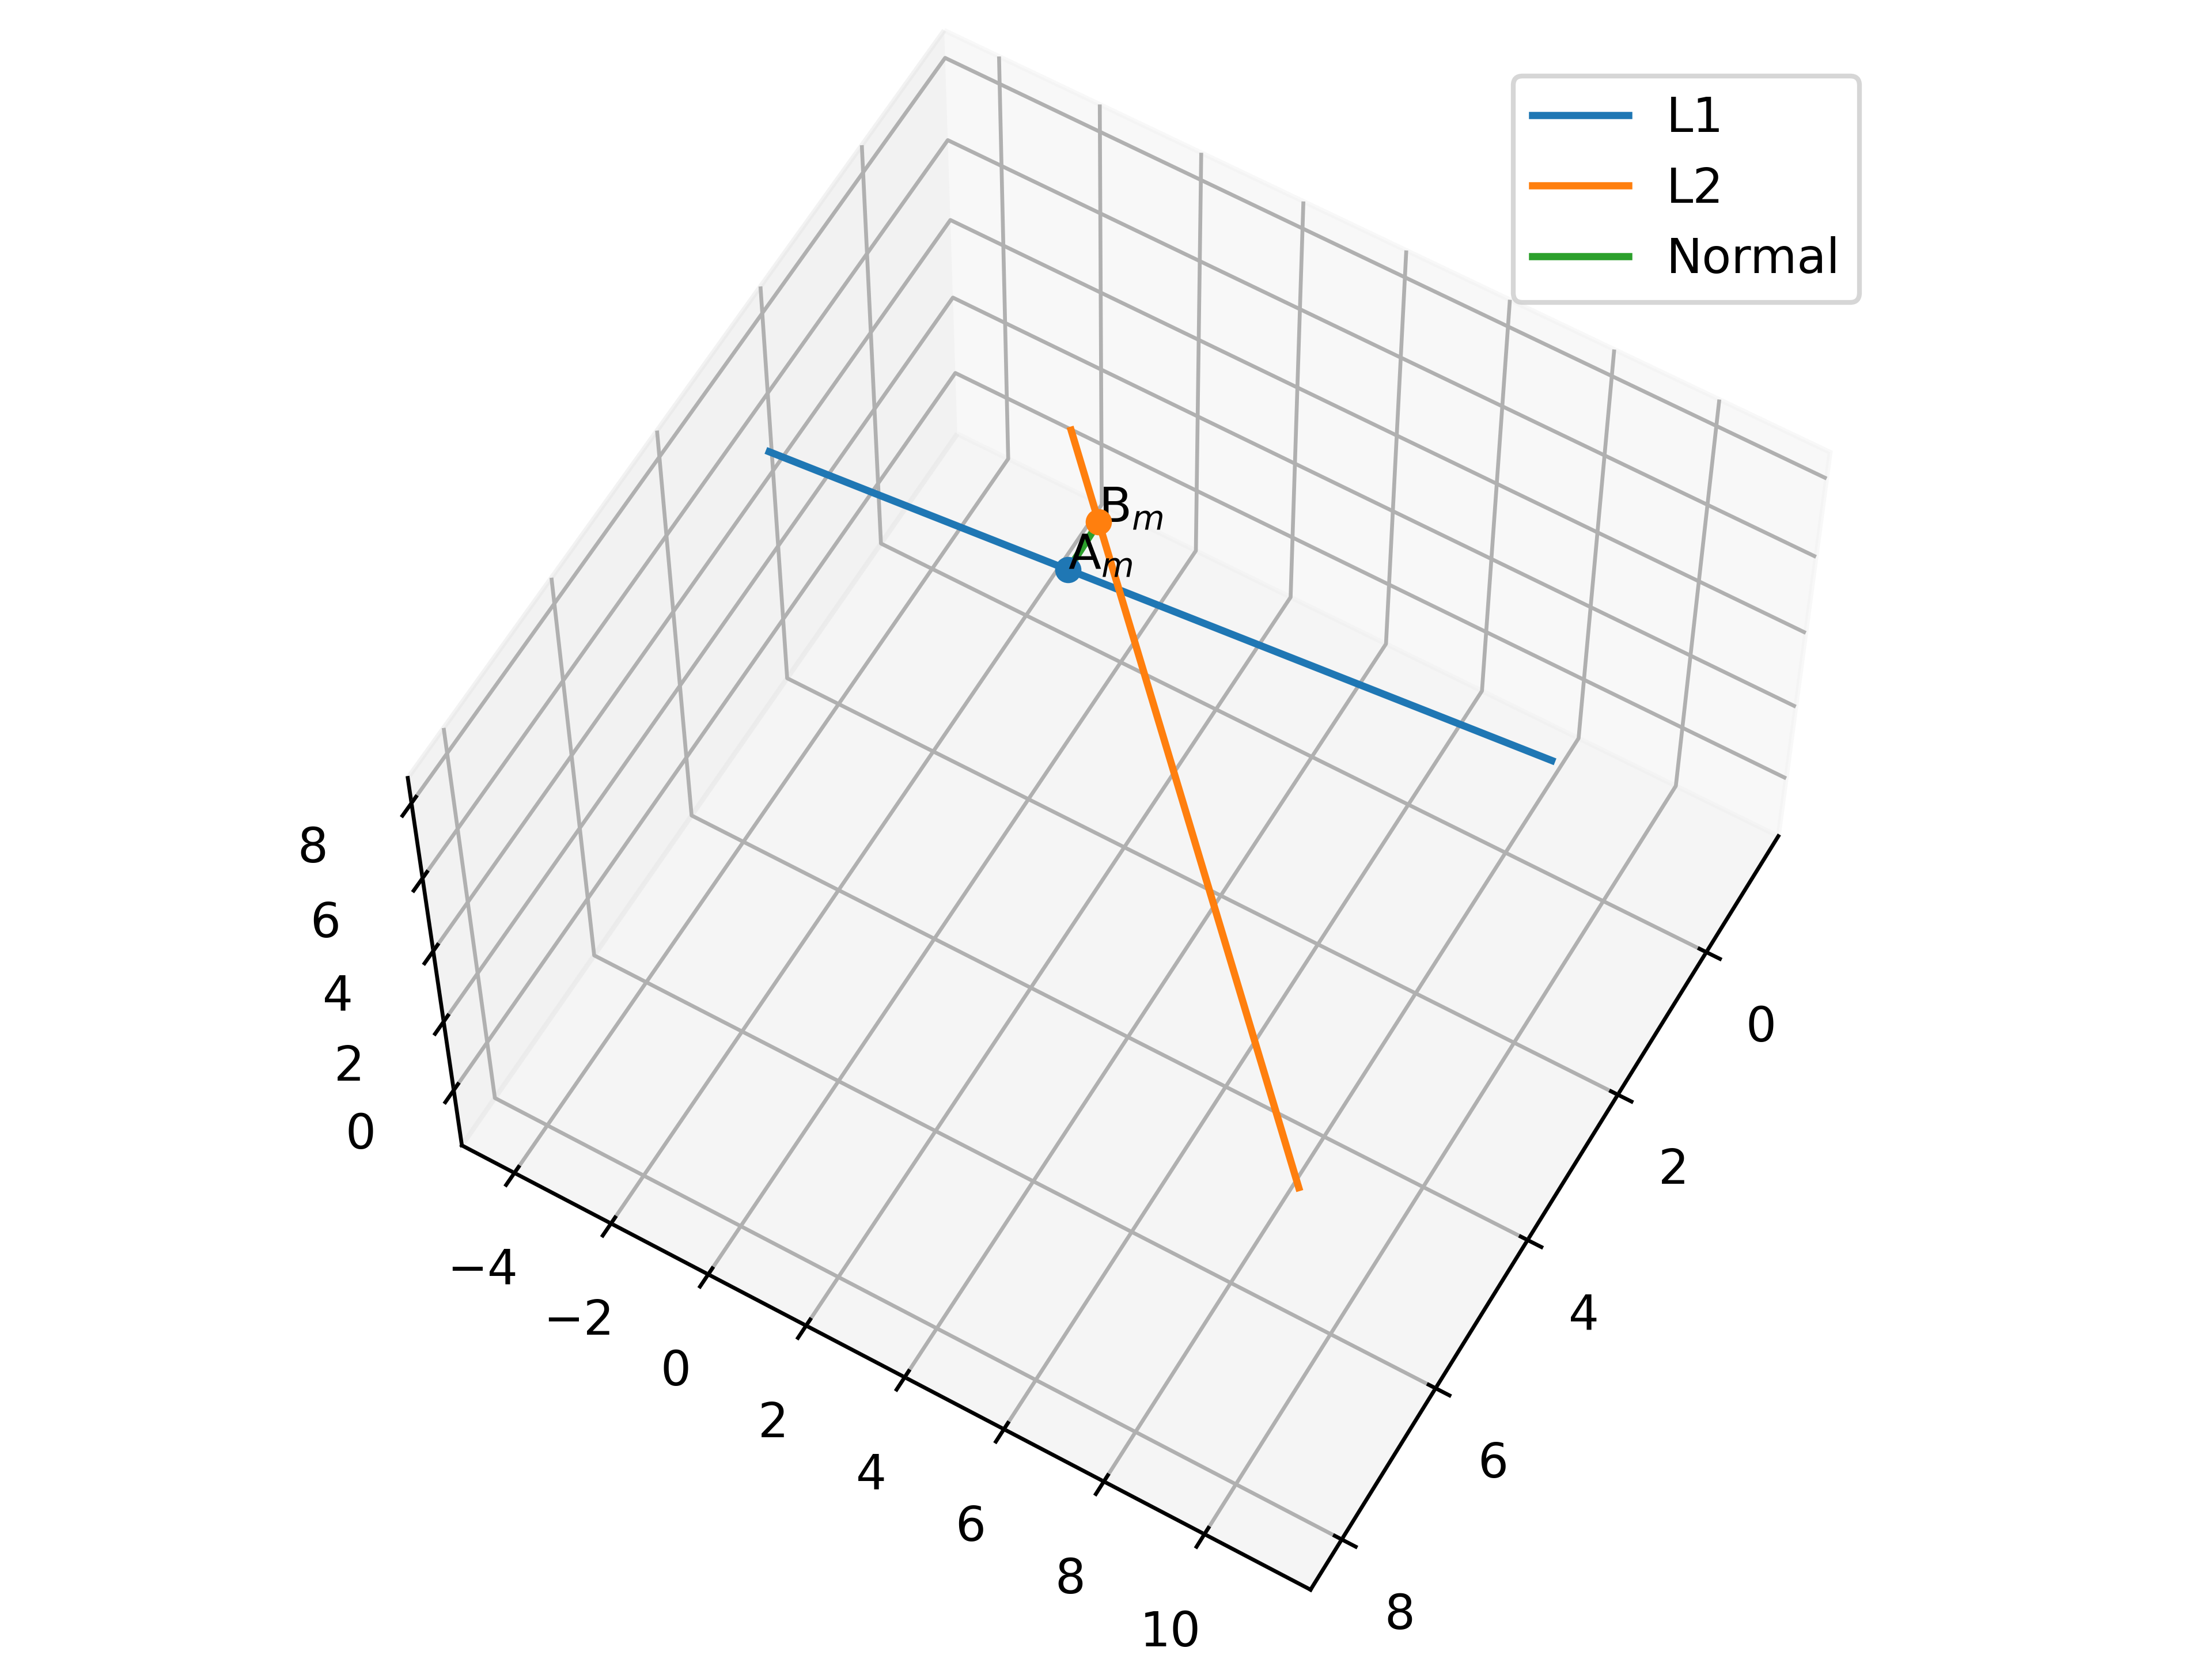
\includegraphics[width=\columnwidth]{chapters/12/11/2/16/svd/figs/skew_svd.png}
        \caption{Finding the shortest distance between two lines using SVD.}
        \label{fig:chapters/12/11/2/16/svd/svd}
    \end{figure}
